\documentclass[11pt]{article}\usepackage[]{graphicx}\usepackage[]{color}
%% maxwidth is the original width if it is less than linewidth
%% otherwise use linewidth (to make sure the graphics do not exceed the margin)
\makeatletter
\def\maxwidth{ %
  \ifdim\Gin@nat@width>\linewidth
    \linewidth
  \else
    \Gin@nat@width
  \fi
}
\makeatother
\usepackage{pdfpages} 
\definecolor{fgcolor}{rgb}{0.345, 0.345, 0.345}
\newcommand{\hlnum}[1]{\textcolor[rgb]{0.686,0.059,0.569}{#1}}%
\newcommand{\hlstr}[1]{\textcolor[rgb]{0.192,0.494,0.8}{#1}}%
\newcommand{\hlcom}[1]{\textcolor[rgb]{0.678,0.584,0.686}{\textit{#1}}}%
\newcommand{\hlopt}[1]{\textcolor[rgb]{0,0,0}{#1}}%
\newcommand{\hlstd}[1]{\textcolor[rgb]{0.345,0.345,0.345}{#1}}%
\newcommand{\hlkwa}[1]{\textcolor[rgb]{0.161,0.373,0.58}{\textbf{#1}}}%
\newcommand{\hlkwb}[1]{\textcolor[rgb]{0.69,0.353,0.396}{#1}}%
\newcommand{\hlkwc}[1]{\textcolor[rgb]{0.333,0.667,0.333}{#1}}%
\newcommand{\hlkwd}[1]{\textcolor[rgb]{0.737,0.353,0.396}{\textbf{#1}}}%
\let\hlipl\hlkwb

\usepackage{ulem}

\usepackage{framed}
\makeatletter
\newenvironment{kframe}{%
 \def\at@end@of@kframe{}%
 \ifinner\ifhmode%
  \def\at@end@of@kframe{\end{minipage}}%
  \begin{minipage}{\columnwidth}%
 \fi\fi%
 \def\FrameCommand##1{\hskip\@totalleftmargin \hskip-\fboxsep
 \colorbox{shadecolor}{##1}\hskip-\fboxsep
     % There is no \\@totalrightmargin, so:
     \hskip-\linewidth \hskip-\@totalleftmargin \hskip\columnwidth}%
 \MakeFramed {\advance\hsize-\width
   \@totalleftmargin\z@ \linewidth\hsize
   \@setminipage}}%
 {\par\unskip\endMakeFramed%
 \at@end@of@kframe}
\makeatother

\definecolor{shadecolor}{rgb}{.97, .97, .97}
\definecolor{messagecolor}{rgb}{0, 0, 0}
\definecolor{warningcolor}{rgb}{1, 0, 1}
\definecolor{errorcolor}{rgb}{1, 0, 0}
\newenvironment{knitrout}{}{} % an empty environment to be redefined in TeX

\usepackage{alltt}
\usepackage{graphicx, fancyhdr}
\usepackage{amsmath, amsfonts}
\usepackage{color}
\usepackage{hyperref}

\newcommand{\blue}[1]{{\color{blue} #1}}

\setlength{\topmargin}{-.5 in} 
\setlength{\textheight}{9 in}
\setlength{\textwidth}{6.5 in} 
\setlength{\evensidemargin}{0 in}
\setlength{\oddsidemargin}{0 in} 
\setlength{\parindent}{0 in}
\newcommand{\ben}{\begin{enumerate}}
\newcommand{\een}{\end{enumerate}}


\lhead{STAT 305}
\chead{Homework \# 4} 
\rhead{Due Thursday, Oct. $3^{rd}$ in the class}
\lfoot{Fall 2019} 
\cfoot{\thepage} 
\rfoot{} 
\renewcommand{\headrulewidth}{0.4pt} 
\renewcommand{\footrulewidth}{0.4pt} 

\def\Exp#1#2{\ensuremath{#1\times 10^{#2}}}
\def\Case#1#2#3#4{\left\{ \begin{tabular}{cc} #1 & #2 \phantom
{\Big|} \\ #3 & #4 \phantom{\Big|} \end{tabular} \right.}
\IfFileExists{upquote.sty}{\usepackage{upquote}}{}
\usepackage{Sweave}
\begin{document}
\Sconcordance{concordance:stat305-hw4.tex:stat305-hw4.Rnw:%
1 83 1 1 0 32 1 1 17 1 1 1 6 55 1}

\pagestyle{fancy} 

Show \textbf{all} of your work on this assignment and answer each question fully in the given context. \\


\emph{Please} staple your assignment!

\begin{enumerate}
	
	\item Chapter 4, Section 1, Exercise 3  (unless directed otherwise you may use JMP; include plots as requested) (page 140) [5 pts each, 25 pts total]
	
	\item Chapter 4, Section 1, Exercise 4  (unless directed otherwise you may use JMP; include plots as requested) (page 140) [5 pts each, 15 pts total]	
	
	\item Chapter 4, Section 2, Exercise 1  (unless directed otherwise you may use JMP; include plots as requested) (page 161) [10 pts]
	
	\item Chapter 4, Section 2, Exercise 2  (unless directed otherwise you may use JMP; include plots as requested; skip part h) (page 161) [5 pts each, 35 pts total]
	



\item
The major cause of axel failure in freight trucks is when shippers exceed the recommended weight limits that can be handled by the axels. 
Issues resulting from these failures have been becoming more frequent as shippers try to cut corners, 
leading members of the state's Department of Transportation to ask one of their civil engineers 
to look into the available data and better advise them on the relationship between excessive weight and axel failure.

A company manufacturing axels provides the engineer with data gathered from conducting experiments loading axels with excessive weight and simulating traveling conditions.
The data consists of two columns, \textbf{excessive weight (in tonnes)} is the amount of weight over the limit that was placed on the axel, and 
\textbf{distance to failure (in tens of thousands of miles)} is the simulated distance to the axel's failure. 

%-- : R code (Code in Document)

\begin{center}
\end{center}

Here are some summaries of the data:

$$
\sum_{i=1}^{50} x_i = 64 \hspace{3cm} \sum_{i=1}^{50} x_i^2 = 107 \\
$$

$$
\sum_{i=1}^{50} y_i = 1996 \hspace{3cm} \sum_{i=1}^{50} y_i^2 = 94078 \\
$$

$$
\sum_{i=1}^{50} x_i y_i = 1982
$$

\begin{enumerate}
       \item  Using the summaries above, fit a linear relationship between \textbf{weight exceeding guidelines} (x) and \textbf{travel distance to failure} (y).[10 pts]
   

      \item Write the equation of the fitted linear relationship. [5 pts] 
      \vspace{2cm}
      \item Find and interpret the value of $R^2$ for the fitted linear relationship.[5 pts]
      \vspace{2cm}
      \item Using the fitted line, provide a predicted value of travel distance to failure when the weight exceeding the guidelines is 3.4 tonnes.[5 pts]
      \vspace{2cm}
      % \item Sketch what you believe the plot of residuals vs weight would look like. Why would this be a problem?[5 pts]
      % \vspace{2cm}

% 
%    \item The JMP output below comes from fitting a quadratic model using $x$ and $x^2$. 
% 
%    \centerline{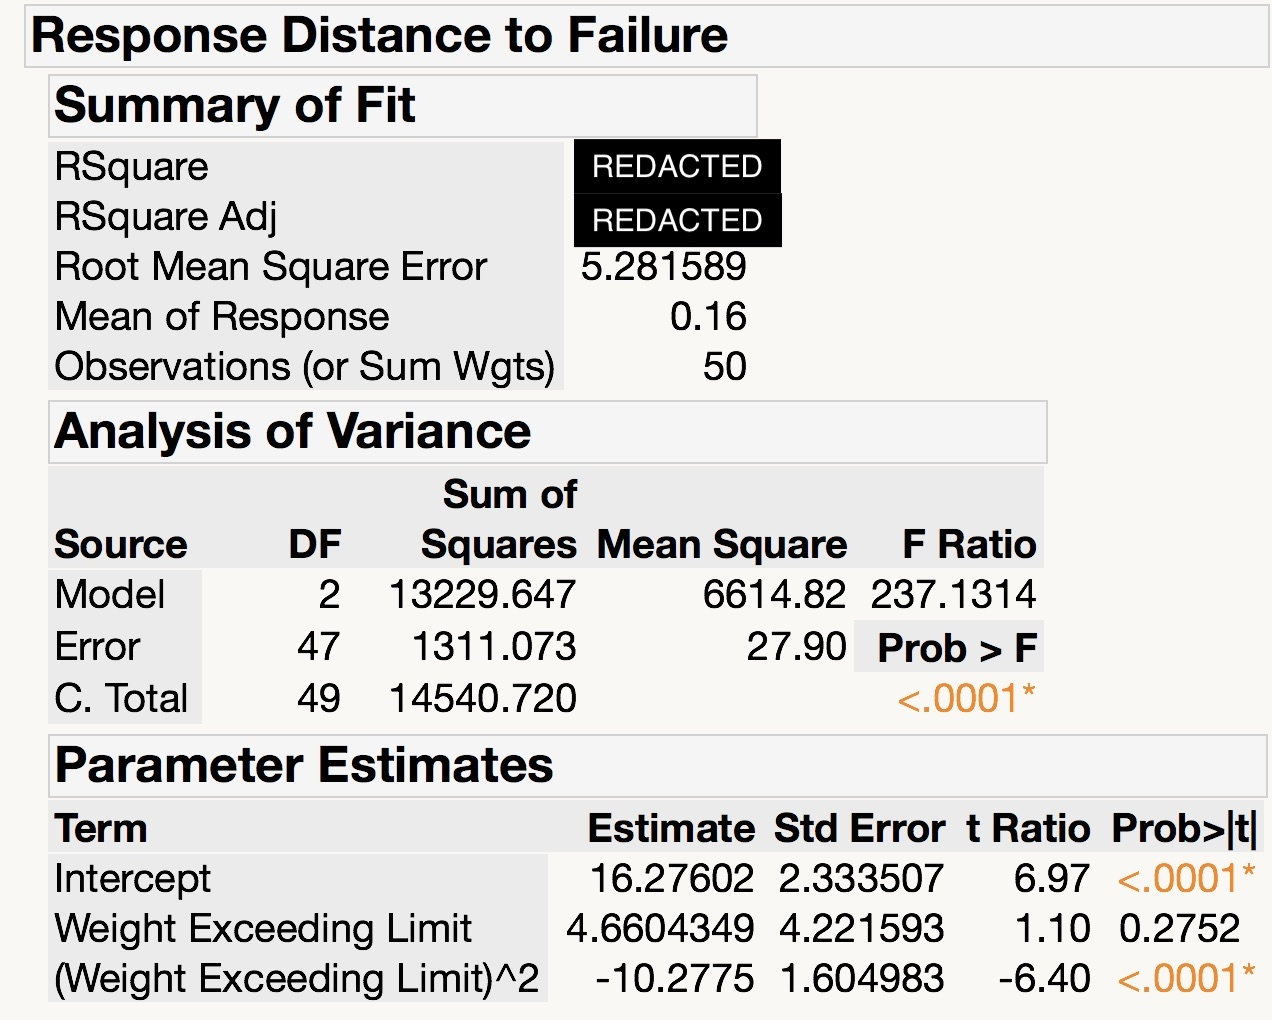
\includegraphics[scale=.2]{FitModel}}
% 
% 
%       \item Write the equation of the fitted quadratic relationship. [5 pts]
%       \vspace{2cm}
%       \item Find and interpret the value of $R^2$ for the fitted quadratic relationship.[5 pts]
%       \vspace{2cm}
%       \item Using the fitted quadratic relationship, provide a predicted value of travel distance to failure when the weight exceeding the guidelines is 3.4 tonnes.[5 pts]

\end{enumerate}

\end{enumerate}	

Total: 100 pts









\end{document}
